\documentclass[10pt]{article}
\usepackage[utf8]{inputenc}
\usepackage{parskip}
\usepackage[margin = 1in]{geometry}
\usepackage{xcolor}
\usepackage[colorlinks = true,linkcolor = blue, urlcolor  = blue,citecolor = blue,anchorcolor = blue]{hyperref}
\usepackage{framed}
\usepackage{apacite}
\usepackage[authoryear,sort]{natbib}
\usepackage{amsmath}
\usepackage{amssymb}
\bibliographystyle{apalike}
\newcommand{\E}{\textrm{E}}
\renewcommand*{\theenumi}{\thesection.\arabic{enumi}}
\renewcommand{\P}{\text{P}}
\usepackage{tikz}
\usetikzlibrary{arrows,shapes.arrows,positioning,shapes,patterns,calc}

\begin{document}

\begin{Large} 
Info 6751. Fall 2022. Problem Set 9. Due on Canvas by 5pm on 31 Oct.
\end{Large}
\hline \vskip .1in

This week, you need time to write ideas for the research proposal (remember---due Oct 31 at 5pm!). The problem set therefore involves only conceptual questions and no coding. You should submit a PDF.

\section{(40 points) Controlled and natural direct effects}

You are studying a treatment $A$ and a mediator $M$. If you use causal notation other than $Y^{a,m}$ and $M^a$, then define your notation.

\begin{enumerate}
    \item (10 points) Write a mathematical statement of the following quantity: the controlled direct effect of treatment (1 vs 0) under an intervention to hold the mediator at the value 1.
    \item (10 points) Write a mathematical statement of the following quantity: the natural direct effect of treatment (1 vs 0) under an intervention to hold the mediator at the value which would have been realized under treatment $A = 0$.
\end{enumerate}
We will consider two settings where you might study these estimands.
\begin{center}
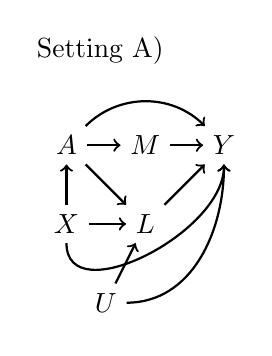
\begin{tikzpicture}
    \node[anchor = north west] at (-.5,1.5) {Setting A)};
    \node (x) at (0,-1) {$X$};
    \node (a) at (0,0) {$A$};
    \node (l) at (1,-1) {$L$};
    \node (m) at (1,0) {$M$};
    \node (y) at (2,0) {$Y$};
    \draw[->, thick] (a) to[bend left = 45] (y);
    \draw[->, thick] (m) -- (y);
    \draw[->, thick] (a) -- (m);
    \draw[->, thick] (a) -- (l);
    \draw[->, thick] (x) -- (a);
%    \draw[->, thick] (l) -- (m);
    \draw[->, thick] (x) -- (l);
    \draw[->, thick] (x) to[out = 270, in = 270] (y);
    \draw[->, thick] (l) -- (y);
    \node (u) at (.5,-2) {$U$};
    \draw[->, thick] (u) -- (l);
    \draw[->, thick] (u) to[out = 0, in = 270](y);
    \node at (0,-2.2) {};
\end{tikzpicture}
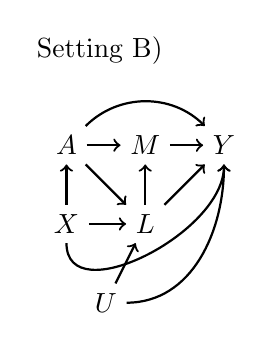
\begin{tikzpicture}
    \node[anchor = north west] at (-.5,1.5) {Setting B)};
    \node (x) at (0,-1) {$X$};
    \node (a) at (0,0) {$A$};
    \node (l) at (1,-1) {$L$};
    \node (m) at (1,0) {$M$};
    \node (y) at (2,0) {$Y$};
    \draw[->, thick] (a) to[bend left = 45] (y);
    \draw[->, thick] (m) -- (y);
    \draw[->, thick] (a) -- (m);
    \draw[->, thick] (a) -- (l);
    \draw[->, thick] (x) -- (a);
    \draw[->, thick] (l) -- (m);
    \draw[->, thick] (x) -- (l);
    \draw[->, thick] (x) to[out = 270, in = 270] (y);
    \draw[->, thick] (l) -- (y);
    \node (u) at (.5,-2) {$U$};
    \draw[->, thick] (u) -- (l);
    \draw[->, thick] (u) to[out = 0, in = 270](y);
    \node at (0,-2.2) {};
\end{tikzpicture}
\end{center}
\begin{enumerate} \setcounter{enumi}{2}
    \item (10 points) Can the controlled direct effect be identified in Setting A, Setting B, neither, or both Settings A and B?
    \item (10 points) Can the natural direct effect be identified in Setting A, Setting B, neither, or both Settings A and B?
\end{enumerate}

\section{(10 points) A common mediation error}

A political scientist randomizes a treatment $A$: some registered voters get cards in the mail telling them the importance of voting, while others do not. All individuals in the study then receive a mail survey collecting data on a mediator $M$: whether they are interested in political affairs (yes or no). Finally, using administrative records, the researcher measures an outcome $Y$: whether the individual votes in the next election. For simplicity, assume we get data for ($A,M,Y$) for all sampled individuals (no non-response).

The researcher asks a research question involving mediation: is there a direct effect of the treatment on voting that does not operate through an effect on interest in political affairs? To answer this question, the researcher estimates an OLS model for $Y$ as a function of $A$ and $M$, and looks at the coefficient on $M$.\footnote{I've added some details, but this general example comes from p.~203 of a good methods paper: Green, D. P., Ha, S. E., & Bullock, J. G. (2010). \href{https://doi.org/10.1177/0002716209351526}{\blue{Enough already about “black box” experiments: Studying mediation is more difficult than most scholars suppose.}} The Annals of the American Academy of Political and Social Science, 628(1), 200-208.}

\clearpage
The DAG below illustrates this setting.

\begin{center}
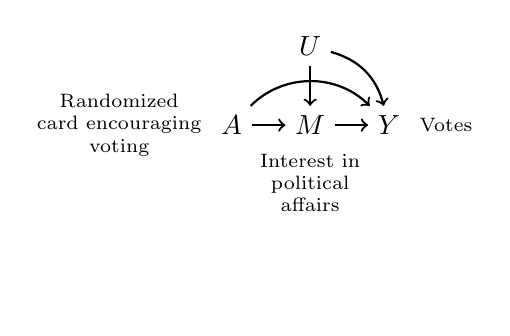
\begin{tikzpicture}
    \node (a) at (0,0) {$A$};
    \node (l) at (1,1) {$U$};
    \node (m) at (1,0) {$M$};
    \node (y) at (2,0) {$Y$};
    \node[anchor = east, align = center, font = \scriptsize] at (a.west) {Randomized\\card encouraging\\voting};
    \node[anchor = north, align = center, font = \scriptsize] at (m.south) {Interest in\\political\\affairs};
    \node[anchor = west, align = center, font = \scriptsize] at (y.east) {Votes};
    \draw[->, thick] (a) to[bend left = 45] (y);
    \draw[->, thick] (m) -- (y);
    \draw[->, thick] (a) -- (m);
    \draw[->, thick] (l) -- (m);]
    \draw[->, thick] (l) to[bend left] (y);
    \node at (0,-2.2) {};
\end{tikzpicture}
\end{center}

\begin{enumerate}
    \item (10 points) Explain to the political scientist how their attempt at mediation has undermined the validity of their experiment. You might refer to the unobserved $U$.
\end{enumerate}

\end{document}

